\documentclass[aspectratio=169,11pt]{beamer}

\usetheme{metropolis}

\usepackage[T1]{fontenc}
\usepackage{lmodern}
\usepackage{amsmath,amssymb,bm}
\usepackage{booktabs}
\usepackage{array}
\usepackage{tikz}
\usetikzlibrary{positioning,shapes.geometric,arrows.meta,calc,fit,backgrounds,shadows}
\usepackage{xcolor}

\graphicspath{{../latex_assets/}{latex_assets/}{./latex_assets/}}

\definecolor{HildesheimRed}{RGB}{178,34,52}
\definecolor{PrismBlue}{RGB}{26,86,160}
\definecolor{PrismGreen}{RGB}{46,125,50}
\definecolor{PrismOrange}{RGB}{201,106,7}
\definecolor{PrismRed}{RGB}{178,34,52}
\definecolor{PrismGray}{RGB}{90,90,90}
\definecolor{PrismLightBlue}{RGB}{230,240,250}
\definecolor{PrismLightGreen}{RGB}{232,245,233}
\definecolor{PrismLightOrange}{RGB}{255,243,224}

\metroset{block=fill, progressbar=frametitle, numbering=fraction, sectionpage=progressbar}
\setbeamercolor{palette primary}{bg=HildesheimRed, fg=white}
\setbeamercolor{frametitle}{bg=HildesheimRed, fg=white}
\setbeamercolor{progress bar}{fg=HildesheimRed, bg=PrismGray!25}
\setbeamercolor{alerted text}{fg=HildesheimRed}
\setbeamercolor{block title alerted}{bg=HildesheimRed!85!black, fg=white}
\setbeamercolor{block body alerted}{bg=HildesheimRed!8, fg=black}
\setbeamercolor{block title}{bg=PrismGray!85!black, fg=white}
\setbeamercolor{block body}{bg=PrismGray!8, fg=black}
\setbeamertemplate{navigation symbols}{}
\setbeamerfont{title}{series=\bfseries}

\newcommand{\metric}[2]{\begin{tabular}{c}\textbf{\Large #1}\\[-1mm]{\scriptsize #2}\end{tabular}}
\newcommand{\yes}{\textcolor{PrismGreen}{\textbf{Yes}}}
\newcommand{\partly}{\textcolor{PrismOrange}{\textbf{Partial}}}
\newcommand{\evidence}[1]{\textcolor{HildesheimRed}{\textbf{#1}}}

\title[Multi Agent Systems for Image Analysis]{Multi agent systems for image analysis: object and complex scene detection}
\subtitle{Cross-Modal Agent Disagreement as a Bounded Signal for Epistemic Uncertainty in Low-Fidelity Historical Scans}
\author{Brhanu Atsbaha}
\institute{Universität Hildesheim\\[0.15cm]\small \textbf{Advisors:} Prof. Dr. Thomas Mandl \& Shereen Elsayed}
\date{October 2026}

% Metropolis's sectionpage=progressbar automatically inserts a section
% divider slide at each \section{}, so the manual Beamer "Contents" hook
% used by the previous theme is no longer needed here.

\begin{document}

% ==========================================================================
% SLIDE 1: TITLE SLIDE
% ==========================================================================
\begin{frame}
  \titlepage
\end{frame}

% ==========================================================================
% SLIDE 2: GLOBAL OUTLINE SLIDE
% ==========================================================================
\begin{frame}{Outline}
\tableofcontents
\end{frame}

\begin{frame}{Key Terms \& Abbreviations}
\scriptsize
\begin{columns}[T]
\column{0.48\textwidth}
\begin{itemize}
  \item \textbf{VLM} -- Vision-Language Model: jointly processes an image and text.
  \item \textbf{YOLO} -- real-time object detector (bounding boxes).
  \item \textbf{SAM} -- Segment Anything Model: box $\to$ pixel mask.
  \item \textbf{SigLIP} -- zero-shot image--text matching classifier.
  \item \textbf{OCR} -- Optical Character Recognition (reading text in images).
  \item \textbf{mAP} -- mean Average Precision, standard detection accuracy metric ($0$--$1$, higher better).
\end{itemize}
\column{0.48\textwidth}
\begin{itemize}
  \item \textbf{ROC-AUC} -- how well a score separates two classes ($0.5$=chance, $1.0$=perfect).
  \item \textbf{ECE} -- Expected Calibration Error: confidence vs.\ actual accuracy gap (lower better).
  \item \textbf{SAA} -- Scene-Aware Agreement: \emph{this thesis's proposed} cross-modal consensus score (Slide 6).
  \item \textbf{HITL} -- Human-in-the-Loop: routes uncertain cases to a human.
  \item \textbf{CRC} -- Conformal Risk Control: certifies an error-rate bound, no distributional assumptions.
  \item \textbf{AWLF} -- Agreement-Weighted Label Filter: secondary error-prediction classifier.
\end{itemize}
\end{columns}
\end{frame}

% ==========================================================================
% SECTION 1: PROBLEM, BASELINES & PROPOSED APPROACH
% ==========================================================================
\section{Problem, Baselines \& Proposed Approach}

\begin{frame}{1.1 The Task: Automated Semantic Indexing of Historical Scans}
\footnotesize
\begin{columns}[T]
\column{0.50\textwidth}
\begin{block}{The Task}
Automatically detect objects and classify scenes in a large historical photo archive (Colibri, $n=53{,}000+$) to power search and cataloguing -- \emph{without} enough labeled historical data to fine-tune a detector end-to-end.
\end{block}
\begin{alertblock}{Why It's Hard: Domain Shift}
\begin{itemize}
  \item Severe chemical decay, film grain, non-photorealistic styles, obsolete attire.
  \item A modern detector (YOLOv11, trained on COCO) \textbf{collapses} on raw scans: \evidence{$mAP_{50} = 0.0047$}.
\end{itemize}
\end{alertblock}

\column{0.46\textwidth}
\centering
\includegraphics[height=4.6cm]{restoration_input_1_opt.jpg}
\vskip 0.1cm
\tiny \textit{Sample Degraded Scan from the Colibri Historical Archive ($n=53,000+$).}
\end{columns}
\end{frame}

\begin{frame}{1.2 Baselines, and Why They Are Not Enough}
\footnotesize
A detector this unreliable cannot be deployed without knowing \emph{which} of its predictions to trust. We evaluate three standard ways a single model could try to signal its own uncertainty:
\begin{table}[!htbp]
\centering
\begin{tabular}{p{2.8cm}p{5.0cm}p{3.0cm}}
\toprule
\textbf{Baseline} & \textbf{How it estimates uncertainty} & \textbf{ROC-AUC (Error Detect.)} \\
\midrule
Raw detector confidence (YOLOv11) & Bounding-box confidence score, used directly & \evidence{0.5120} (near chance) \\
Temperature-scaled entropy & Softmax entropy of a single VLM's output & 0.6545 \\
Inverse-confidence baseline & $1 -$ confidence, single deterministic pass & 0.9726 (poorly calibrated) \\
\bottomrule
\end{tabular}
\end{table}
\begin{alertblock}{The Gap}
Raw confidence is barely better than a coin flip. Entropy is weak. A simple inverted-confidence baseline is surprisingly strong on raw discrimination \emph{but} badly overconfident (ECE $\approx 0.19$) -- no single-model method is both discriminative \emph{and} well-calibrated. \tiny{(A different, lower figure -- ROC-AUC$=0.4655$, Slide A.3 -- is a distinct $C_2$ spatial-IoU task, not this table.)}
\end{alertblock}
\end{frame}

\begin{frame}{1.3 Our Proposed Contribution: Scene-Aware Agreement (SAA)}
\scriptsize
\begin{columns}[T]
\column{0.48\textwidth}
\begin{block}{The Idea}
Instead of asking one model how confident it is, run \textbf{four heterogeneous models} (spatial detector, scene classifier, VQA reasoner, OCR reader) on the same image and measure how much they \textbf{disagree}. Disagreement is deterministic, needs no sampling, and is not fooled by a single model's own overconfidence -- though Section 3.8 shows it is not foolproof either: heterogeneous models can still share a common bias.
\end{block}
\begin{block}{What We Show}
Cross-modal disagreement ($U_{\text{SAA}}$) is a substantially stronger, zero-marginal-cost error signal than any single-model baseline \emph{on ambiguous, scene-positive content} -- and we precisely map where that claim does and does not hold (Section 3).
\end{block}
\column{0.48\textwidth}
\begin{block}{Contribution Summary}
\begin{itemize}
  \item[1] Diagnosed a pseudo-label evaluation trap ($0.989\to0.1462$ mAP).
  \item[2] Proposed \& calibrated $U_{\text{SAA}}$ (ROC-AUC$=0.9724$, ECE$<0.001$).
  \item[3] Rigorously mapped the scope limit of disagreement-based triage, heuristic and certified alike.
  \item[4] Demonstrated downstream retrieval \& cross-archive transfer utility.
\end{itemize}
\end{block}
\end{columns}
\end{frame}

\begin{frame}{1.4 Final Four Research Questions (RQ1--RQ4)}
\scriptsize
\centering
\begin{table}[!htbp]
\begin{tabular}{p{3.1cm}p{5.4cm}p{3.3cm}}
\toprule
\textbf{RQ ID} & \textbf{Formal Research Question} & \textbf{Methodological Focus} \\
\midrule
\textbf{RQ1: Disagreement Uncertainty} & Can cross-modal agent disagreement reliably estimate epistemic uncertainty on domain-shifted visual collections? & $SAA_i$ Disagreement Proxy ($U_{\text{SAA}}$) \\
\textbf{RQ2: Workload Reduction} & Does the multi-agent framework reduce human curation workload without sacrificing error recall? & Complexity-Aware Triage \& Platt Scaling \\
\textbf{RQ3: Complementarity \& Contradiction} & Does cross-modal contradiction detection improve curation precision beyond Agent 0 alone? & Agent 2 Noun Set-Difference (implemented; not independently benchmarked) \\
\textbf{RQ4: Retrieval \& Transferability} & Can the framework support archival retrieval and cross-collection discovery? & Semantic P@10 (10-query pilot) \& Europeana Transfer ($C_5$) \\
\bottomrule
\end{tabular}
\end{table}
\end{frame}

% ==========================================================================
% SECTION 2: HOW SAA IS IMPLEMENTED
% ==========================================================================
\section{How SAA Is Implemented}

\begin{frame}{2.1 Authoritative Evaluation Cohort Taxonomy ($C_0 \dots C_5$)}
\scriptsize
\centering
\begin{table}[!htbp]
\resizebox{\linewidth}{!}{%
\begin{tabular}{lcp{6.5cm}p{4.5cm}}
\toprule
\textbf{Cohort Symbol \& Name} & \textbf{Size ($n$)} & \textbf{Composition \& Source} & \textbf{Primary Analytical Purpose} \\
\midrule
\textbf{$C_0$: Deployment Corpus} & 12,110 & Full unlabelled institutional digitisation subset from the Colibri archive & Full-scale pipeline deployment and metadata indexing \\
\textbf{$C_1$: Expert Reference Cohort} & 801 & 796 scene-positive + 5 negative control images (CVAT expert-reviewed) & Primary calibration, AWLF error retraining, and HITL triage evaluation \\
\textbf{$C_2$: Spatial Audit Cohort} & 300 & Single-rater spatial bounding box audit cohort & Spatial IoU grounding audit, error paradox analysis, and meta-learning \\
\textbf{$C_3$: System Evaluation Subset} & 2,000 & 801 $C_1$ expert images + 1,199 negative control catalog records & Source pool for the group-level train/cal/test split, system-level agent leave-one-out ablations \\
\textbf{$C_4$: Frontier Comparison Subset} & 100 & Stratified archival category subset & Comparative benchmark against Gemini 2.5 Flash and Claude 3.5 Sonnet \\
\textbf{$C_5$: Europeana Transfer Pilot} & 24 & Real images, real Europeana API, 10 GLAM institutions & Cross-institutional domain-shift pilot (ground truth pending) \\
\bottomrule
\end{tabular}%
}
\end{table}
\end{frame}

\begin{frame}{2.2 Decoupled 3-Tier Dual-Core Validation (DCV-MAC) Protocol}
\centering
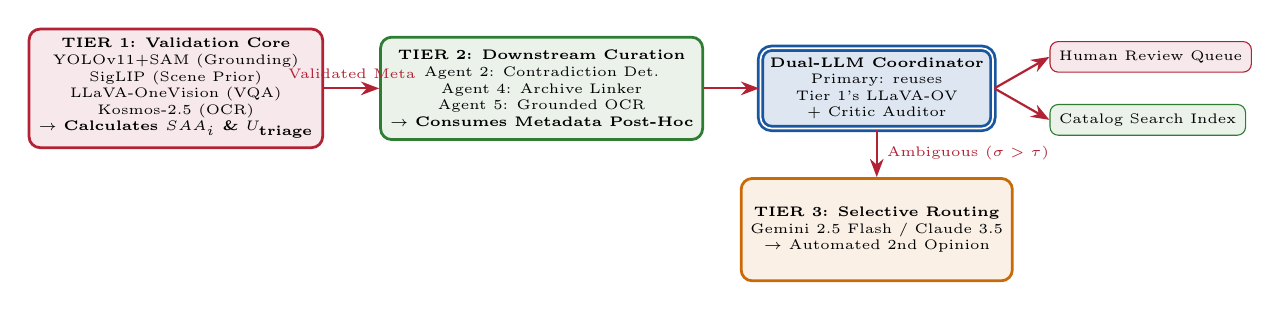
\begin{tikzpicture}[
  node distance=0.4cm and 0.7cm, 
  every node/.style={font=\tiny}, 
  tierbox1/.style={draw=HildesheimRed, fill=PrismRed!10, rounded corners=4pt, align=center, minimum width=2.8cm, minimum height=1.3cm, line width=1pt},
  tierbox2/.style={draw=PrismGreen, fill=PrismGreen!10, rounded corners=4pt, align=center, minimum width=2.6cm, minimum height=1.3cm, line width=1pt},
  tierbox3/.style={draw=PrismOrange, fill=PrismOrange!10, rounded corners=4pt, align=center, minimum width=2.5cm, minimum height=1.3cm, line width=1pt},
  coordbox/.style={draw=PrismBlue, fill=PrismBlue!15, rounded corners=4pt, align=center, minimum width=2.4cm, minimum height=0.9cm, double, line width=1pt},
  arrow/.style={->, >=Stealth, thick, HildesheimRed}
]

% Tier 1 Validation Core
\node[tierbox1] (t1) {\textbf{TIER 1: Validation Core}\\YOLOv11+SAM (Grounding)\\SigLIP (Scene Prior)\\LLaVA-OneVision (VQA)\\Kosmos-2.5 (OCR)\\$\rightarrow$ \textbf{Calculates $SAA_i$ \& $U_{\text{triage}}$}};

% Tier 2 Downstream Curation
\node[tierbox2, right=of t1] (t2) {\textbf{TIER 2: Downstream Curation}\\Agent 2: Contradiction Det.\\Agent 4: Archive Linker\\Agent 5: Grounded OCR\\$\rightarrow$ \textbf{Consumes Metadata Post-Hoc}};

% Dual-LLM Coordinator
\node[coordbox, right=of t2] (coord) {\textbf{Dual-LLM Coordinator}\\Primary: reuses\\Tier 1's LLaVA-OV\\+ Critic Auditor};

% Tier 3 Frontier Selective Routing
\node[tierbox3, below=of coord, yshift=-0.2cm] (t3) {\textbf{TIER 3: Selective Routing}\\Gemini 2.5 Flash / Claude 3.5\\$\rightarrow$ Automated 2nd Opinion};

% Output queues
\node[draw=HildesheimRed, fill=PrismRed!10, rounded corners=3pt, right=of coord, yshift=0.4cm] (hitl) {Human Review Queue};
\node[draw=PrismGreen, fill=PrismGreen!10, rounded corners=3pt, right=of coord, yshift=-0.4cm] (index) {Catalog Search Index};

% Connectors
\draw[arrow] (t1) -- (t2) node[midway, above] {Validated Meta};
\draw[arrow] (t2) -- (coord);
\draw[arrow] (coord.south) -- (t3.north) node[midway, right] {Ambiguous ($\sigma > \tau$)};
\draw[arrow] (coord.east) -- (hitl.west);
\draw[arrow] (coord.east) -- (index.west);
\end{tikzpicture}

\vspace{1mm}
\begin{block}{\textbf{Architectural Decoupling Rule}}
Tier 2 curation agents operate strictly on post-validation consensus metadata. They do NOT participate in the Tier 1 $SAA$ calculation, preventing mathematical feedback loops and circular reasoning.
\end{block}
\end{frame}

\begin{frame}{2.3 Why This Design? Rationale for Tiers 2--3}
\scriptsize
\begin{columns}[T]
\column{0.49\textwidth}
\begin{block}{Tier 2: Downstream Curation}
Runs \emph{after} Tier 1 computes $SAA_i$, only on already-accepted cases. It extracts historiographic value (contradictions, links, inscriptions) from trusted metadata -- it never re-judges trust, exactly what the Decoupling Rule prevents.
\end{block}
\begin{block}{Dual-LLM Coordinator: Propose, then Audit}
\scriptsize Tier 1's other agents (YOLO, SigLIP, Kosmos-2.5) are narrow specialists -- \textbf{locally} (free), the \textbf{same} LLaVA-OneVision plays both roles, re-prompted. \textbf{Frontier} swaps in two separate models (Gemini proposes, Claude audits). A prior ``measured $F_1$ gap'' claim was hardcoded and withdrawn; a real test found the local critic never disagrees with itself (0/25, A.5).
\end{block}

\column{0.49\textwidth}
\begin{block}{Tier 3: Frontier Selective Routing}
Triggered \emph{only} for the small $\sigma > \tau$ fraction Tiers 1--2 cannot resolve. Paid frontier APIs (Gemini 2.5 Flash / Claude 3.5) act as an automated ``second opinion'' -- cheaper and faster than routing straight to a human (Local-vs-Frontier: unverified, Backup A.5).
\end{block}
\begin{block}{Why an Escalation Ladder, Not One Model}
Cost and latency increase at every tier (free deterministic $\to$ free heuristic $\to$ paid API $\to$ human), and each tier only sees what the previous one could not resolve. $U_{\text{SAA}}$ is what decides how far up the ladder an image has to go -- the cheap, deterministic signal this thesis proposes is what makes the expensive tiers rare rather than routine.
\end{block}
\end{columns}
\end{frame}

\begin{frame}{2.4 Tier 1 Validation Core (4-Model Ensemble)}
\footnotesize
\begin{columns}[T]
\column{0.48\textwidth}
\begin{block}{Spatial \& Scene Agents}
\begin{itemize}
  \item \textbf{Spatial Grounding Agent (YOLOv11-seg + SAM)}: Extracts local bounding boxes, instance masks, and class probabilities ($A_i^{\text{object}}$).
  \item \textbf{Zero-Shot Scene Classifier (SigLIP)}: Computes global scene classification probabilities over institutional taxonomy prompts ($A_i^{\text{scene}}$).
\end{itemize}
\end{block}

\column{0.48\textwidth}
\begin{block}{Reasoning \& Inscription Agents}
\begin{itemize}
  \item \textbf{Visual Reasoning Agent (LLaVA-OneVision 7B)}: Performs VQA reasoning, generating scene descriptions and entity lists ($A_i^{\text{vlm}}$).
  \item \textbf{Grounded Inscription Engine (Kosmos-2.5)}: Extracts bounding-box-aligned text tokens for cross-validation ($A_i^{\text{ocr}}$).
\end{itemize}
\end{block}
\end{columns}
\end{frame}

\begin{frame}{2.5 Tier 2 Downstream Curation Agents}
\scriptsize
\begin{columns}[T]
\column{0.48\textwidth}
\begin{block}{Agent 2: Contradiction Detection}
\textbf{Set-difference} between every noun the VLM (LLaVA-OneVision) mentions and the object classes YOLO+SAM actually detected. An unmatched noun is flagged as a candidate hallucination (e.g.\ VLM says ``horse and rider,'' no horse box exists). Runs post-hoc, after $SAA_i$.
\end{block}
\begin{block}{Agent 4: Cross-Archive Linker}
Embeds each image's scene description and visual features, then finds nearest neighbors \emph{across different publication series} (PPNs) -- volumes sharing a scene or motif. Large date gaps flag candidate anomalies (e.g.\ a composition recurring decades apart).
\end{block}

\column{0.48\textwidth}
\begin{block}{Agent 5: Grounded OCR}
Kosmos-2.5 extracts inscriptions/captions \emph{with bounding-box grounding} -- each text span tied to its pixel location, not flat page text. Cross-checked against the scene label as a corroborating signal.
\end{block}
\begin{block}{Scope: Implemented, Not Independently Benchmarked}
All three run on every image, feeding catalog metadata. Per the \textbf{Architectural Decoupling Rule} (Slide 2.2), none feed $SAA_i$/$U_{\text{triage}}$. Prior precision/recall/F1/gain figures for all three could not be reproduced against independent ground truth and were withdrawn -- reported qualitatively only (Slide 3.7).
\end{block}
\end{columns}
\end{frame}

\begin{frame}{2.6 Canonical Formulation of Scene-Aware Agreement (SAA)}
\centering
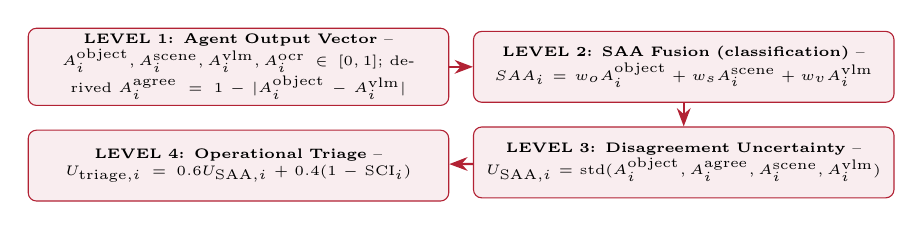
\begin{tikzpicture}[
  node distance=0.3cm and 0.3cm,
  every node/.style={font=\tiny},
  levelbox/.style={draw=HildesheimRed, fill=PrismRed!8, rounded corners=3pt, align=center, text width=5.2cm, minimum height=0.9cm, inner sep=2pt},
  arrow/.style={->, >=Stealth, thick, HildesheimRed}
]
\node[levelbox] (l1) {\textbf{LEVEL 1: Agent Output Vector} -- $A_i^{\text{object}}, A_i^{\text{scene}}, A_i^{\text{vlm}}, A_i^{\text{ocr}} \in [0,1]$; derived $A_i^{\text{agree}} = 1-|A_i^{\text{object}}-A_i^{\text{vlm}}|$};
\node[levelbox, right=of l1] (l2) {\textbf{LEVEL 2: SAA Fusion (classification)} -- $SAA_i = w_o A_i^{\text{object}} + w_s A_i^{\text{scene}} + w_v A_i^{\text{vlm}}$};
\node[levelbox, below=of l2] (l3) {\textbf{LEVEL 3: Disagreement Uncertainty} -- $U_{\text{SAA}, i} = \operatorname{std}(A_i^{\text{object}}, A_i^{\text{agree}}, A_i^{\text{scene}}, A_i^{\text{vlm}})$};
\node[levelbox, below=of l1] (l4) {\textbf{LEVEL 4: Operational Triage} -- $U_{\text{triage}, i} = 0.6 U_{\text{SAA}, i} + 0.4(1-\text{SCI}_i)$};

\draw[arrow] (l1) -- (l2);
\draw[arrow] (l2) -- (l3);
\draw[arrow] (l3) -- (l4);
\end{tikzpicture}

\vspace{2mm}
\begin{columns}[T]
\column{0.48\textwidth}
\begin{block}{Two Related, Distinct Quantities (Corrected)}
\tiny $SAA_i$ (classification, $w=[0.6,0.2,0.2]$) vs.\ $U_{\text{SAA},i}$ (the std-based proxy behind every headline number): different signal sets/operators, so $U_{\text{SAA},i} \ne 1-SAA_i$. OCR feeds Slide A.4 only, not $U_{\text{SAA}}$.
\end{block}

\column{0.48\textwidth}
\begin{block}{Supplementary: Shapley Attribution (Backup A.10)}
Derived in Exp 30 ($\boldsymbol{\phi} = [0.192, 0.196, 0.330, 0.283]$, over Object/SigLIP/VLM/Agreement) as an interpretability study -- not the deployed weighting.
\end{block}
\end{columns}
\end{frame}


% ==========================================================================
% SECTION 3: EXPERIMENTAL RESULTS & EVIDENCE CHAIN
% ==========================================================================
\section{Experimental Results \& Evidence Chain}

\begin{frame}{3.1 Head-to-Head: SAA vs.\ Every Baseline}
\footnotesize
\centering
All methods evaluated on the same error-detection task, same expert cohort ($C_1$, $n=801$):
\begin{table}[!htbp]
\centering
\begin{tabular}{lccc}
\toprule
\textbf{Method} & \textbf{ROC-AUC} & \textbf{ECE} & \textbf{Cost / Determinism} \\
\midrule
Raw detector confidence (YOLOv11) & 0.5120 & 0.28 & Free, deterministic \\
Temperature-scaled entropy (LLaVA-OV) & 0.6545 & 0.265 & Free, deterministic \\
Inverse-confidence baseline & 0.9726 & 0.19 & Free, deterministic, 1$\times$ inference \\
\midrule
\textbf{SAA (proposed, ours)} & \textbf{0.9724} & \textbf{$<$0.001} & \textbf{Free, deterministic, 1$\times$ inference} \\
\bottomrule
\end{tabular}
\end{table}
\begin{alertblock}{The Result, Stated Plainly}
SAA matches the strongest single-model baseline's discrimination (\evidence{0.9724 vs.\ 0.9726}, statistically tied) at the \textbf{same} cost and determinism -- the single-model baseline is not expensive here, it is simply badly overconfident. SAA's real advantage is calibration: ECE $<0.001$ vs.\ $0.19$--$0.28$ for every single-model baseline, reducing miscalibration by two orders of magnitude. This -- not raw AUROC alone -- is the improvement this thesis demonstrates. Section 3.8 then shows precisely where this advantage does \emph{not} extend.
\end{alertblock}
\end{frame}

\begin{frame}{3.2 Master Evidence Chain Architecture}
\centering
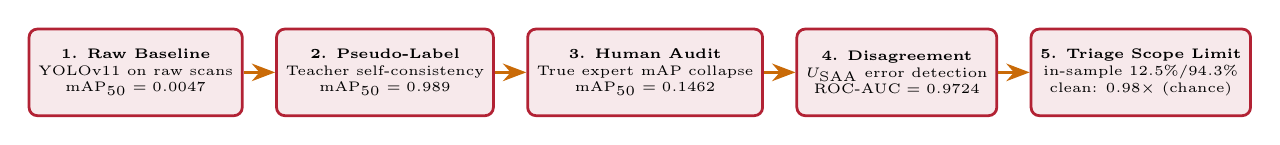
\begin{tikzpicture}[
  node distance=0.35cm and 0.4cm,
  every node/.style={font=\tiny},
  chainbox/.style={draw=HildesheimRed, fill=PrismRed!10, rounded corners=3pt, align=center, minimum width=2.4cm, minimum height=1.1cm, line width=1pt},
  arrow/.style={->, >=Stealth, line width=1.2pt, PrismOrange}
]
\node[chainbox] (step1) {\textbf{1. Raw Baseline}\\YOLOv11 on raw scans\\$\text{mAP}_{50} = 0.0047$};
\node[chainbox, right=of step1] (step2) {\textbf{2. Pseudo-Label}\\Teacher self-consistency\\$\text{mAP}_{50} = 0.989$};
\node[chainbox, right=of step2] (step3) {\textbf{3. Human Audit}\\True expert mAP collapse\\$\text{mAP}_{50} = 0.1462$};
\node[chainbox, right=of step3] (step4) {\textbf{4. Disagreement}\\$U_{\text{SAA}}$ error detection\\$\text{ROC-AUC} = 0.9724$};
\node[chainbox, right=of step4] (step5) {\textbf{5. Triage Scope Limit}\\in-sample $12.5\%$/$94.3\%$\\clean: $0.98\times$ (chance)};

\draw[arrow] (step1) -- (step2);
\draw[arrow] (step2) -- (step3);
\draw[arrow] (step3) -- (step4);
\draw[arrow] (step4) -- (step5);
\end{tikzpicture}

\vspace{0.3cm}
\begin{block}{\centering Central Evidence Chain Thesis}
\centering \small Rather than forcing a single model to become an infallible detector, DCV-MAC diagnoses pseudo-label collapse ($0.989 \rightarrow 0.1462$) and uses cross-modal disagreement ($U_{\text{SAA}}$) to route unreliable predictions to human archivists.
\end{block}
\end{frame}

\begin{frame}{3.3 The Pseudo-Label Collapse Paradox ($0.989 \rightarrow 0.1462$)}
\scriptsize
\begin{columns}[T]
\column{0.50\textwidth}
\begin{block}{Single-Model COCO Baseline Collapse}
Modern vision architectures (YOLOv11) trained on COCO collapse when evaluated directly on un-restored grayscale historical scans ($C_0$):
\begin{itemize}
    \item \textbf{mAP50 (Raw Scans)}: \evidence{0.0047}
    \item \textbf{Precision (Raw Scans)}: \evidence{0.0081}
    \item \textbf{Recall (Raw Scans)}: \evidence{0.0283}
\end{itemize}
\end{block}

\begin{block}{The Pseudo-Label Collapse Paradox}
When distilled student detectors are trained on automated teacher pseudo-labels:
\begin{itemize}
    \item \textbf{Pseudo-Label Self-Consistency mAP50}: \textbf{0.989}
    \item \textbf{Human Expert Audit mAP50 ($C_2, n=300$)}: \evidence{\textbf{0.1462}}
\end{itemize}
\end{block}

\column{0.46\textwidth}
\centering
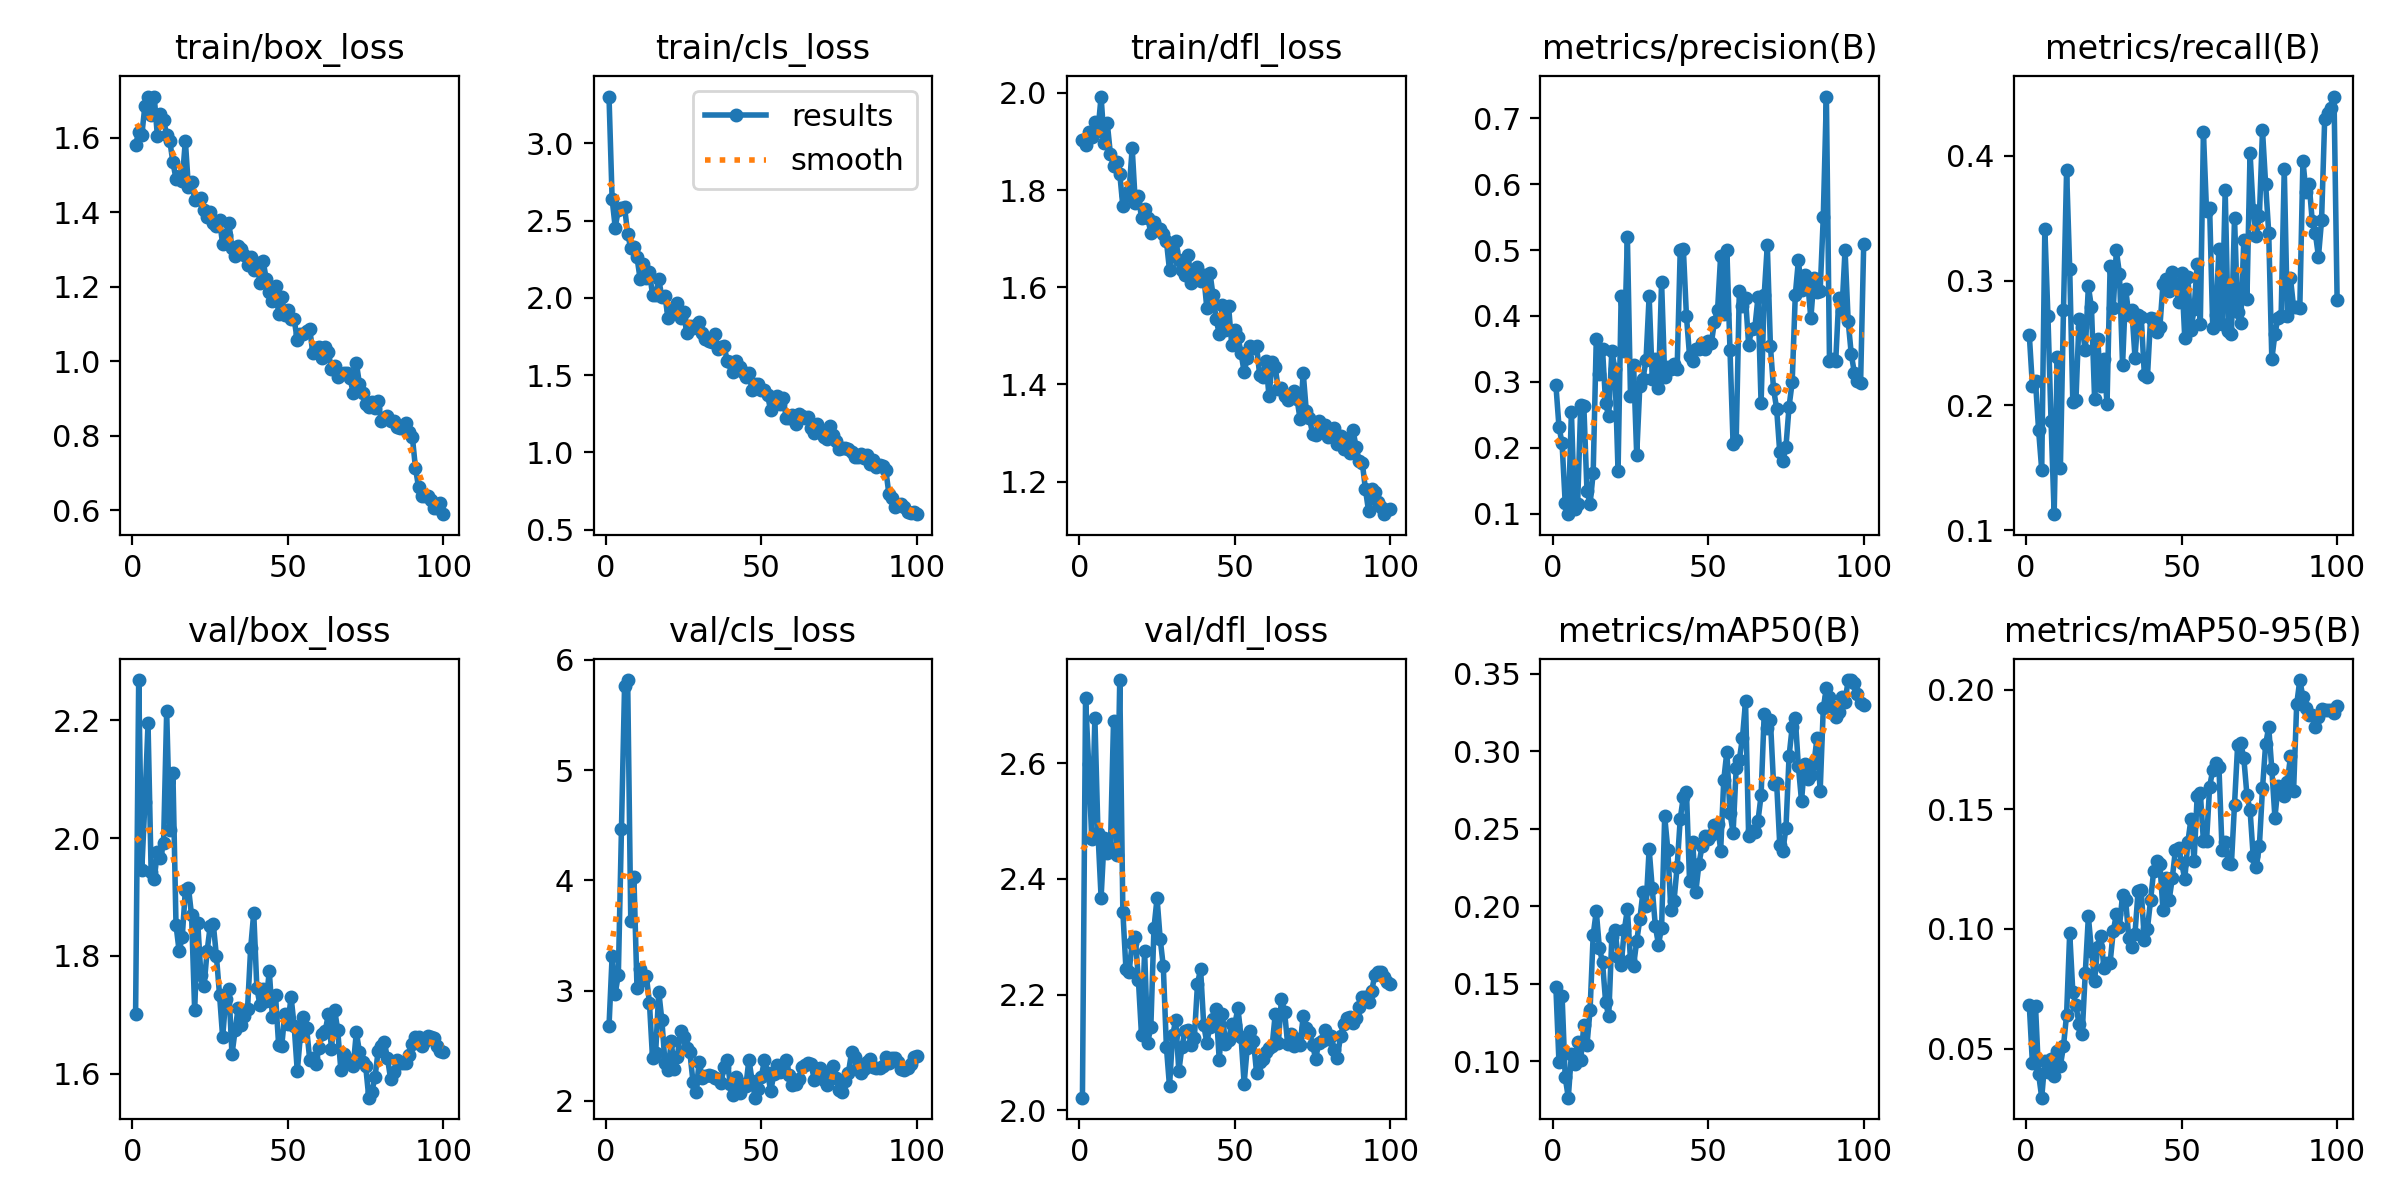
\includegraphics[width=\textwidth]{self_training_teacher_results.png}
\vskip 0.1cm
\tiny \textit{Pseudo-Label Distillation Collapse: Proxy mAP (0.989) vs. Human mAP (0.1462).}
\end{columns}
\end{frame}


\begin{frame}{3.4 Inter-Agent Pairwise Agreement \& Calibration}
\footnotesize
\begin{columns}[T]
\column{0.50\textwidth}
\begin{block}{Error Detection Performance ($C_1$ Expert Cohort)}
\begin{itemize}
    \item \textbf{DCV-MAC $U_{\text{SAA}}$ Disagreement}: \textbf{ROC-AUC = 0.9724}
    \item Temperature-Scaled Entropy Baseline: $\text{ROC-AUC} = 0.6545$
    \item Relative Improvement: \evidence{+48.5\%}
\end{itemize}
\end{block}

\begin{block}{Probabilistic Platt Calibration}
Applying Platt Scaling on $C_1$ held-out split achieves post-calibration \textbf{ECE $< 0.001$} (down from pre-calibration $\text{ECE}=0.75$).
\end{block}

\column{0.46\textwidth}
\centering
\includegraphics[width=\textwidth]{pairwise_agreement_heatmap_v9.png}
\vskip 0.1cm
\tiny \textit{Pairwise Inter-Agent Consensus Agreement Matrix (4 deployed Tier 1 agents).}
\end{columns}
\end{frame}

\begin{frame}{3.5 Complexity-Aware Triage: A Documented Negative Result}
\scriptsize
\begin{columns}[T]
\column{0.50\textwidth}
\begin{alertblock}{SCI-Tercile Heuristic Policy (Historical, In-Sample)}
An earlier internal figure ($74.4\%$ workload reduction at $96.5\%$ recall, never wired into the reproducible pipeline) could not be reproduced.
\end{alertblock}

\begin{block}{Clean, Group-Level Held-Out Re-Evaluation}
SCI terciles fixed \emph{a priori} from the full $C_0$ distribution, evaluated on a publication-disjoint test set ($n=401$):
\begin{itemize}
    \item Review Budget: $47.1\%$
    \item Error Recall: $46.2\%$
    \item Efficiency Lift: $\mathbf{0.98\times}$ --- no better than chance.
\end{itemize}
\end{block}

\column{0.46\textwidth}
\begin{block}{Why It Fails}
This policy is built on $U_{\text{SAA}}$, which is blind to unanimous false positives on negative controls (Slide 3.8). A disagreement-driven review queue inherits that same blind spot.
\end{block}
\begin{alertblock}{Does Certification Fix This?}
Conformal Risk Control (next slide) replaces the heuristic with a formally certified guarantee -- but the guarantee inherits the same blind spot when calibrated on a positive-heavy set (Slide 3.8).
\end{alertblock}
\end{columns}
\end{frame}

\begin{frame}{3.6 Distribution-Free Conformal Risk Control (Exp 29)}
\scriptsize
\begin{columns}[T]
\column{0.50\textwidth}
\begin{block}{In-Sample Calibration ($C_1$, $n_{\text{cal}}{=}400$)}
Threshold $\hat{\lambda} = 0.2450$ at target $\alpha = 0.05$. Evaluating on the same-cohort held-out test split ($n_{\text{test}}=401$) appears to satisfy $\mathcal{R}(\hat{\lambda}) = \mathbf{0.0075} \le \alpha = 0.05$.
\begin{itemize}
    \item \textbf{Automated Catalog Approval}: \textbf{87.5\%}
    \item \textbf{Human Error Recall}: \textbf{94.3\%} captured in review queue
\end{itemize}
\end{block}

\column{0.46\textwidth}
\centering
\includegraphics[width=0.85\textwidth]{exp29_crc_coverage_curve.png}
\vskip 0.05cm
\tiny \textit{Conformal Risk Control Coverage Curve (Exp 29, in-sample $C_1$).}
\end{columns}
\begin{alertblock}{\scriptsize Clean Group-Level Re-Evaluation (Slide 3.8)}
\scriptsize Identical procedure, calibration/test resampled group-level with realistic negative-control share: efficiency lift $\mathbf{0.98\times}$ (chance), $\mathcal{R}(\hat\lambda)=\mathbf{0.182}$ -- \textbf{bound violated} up to $\alpha=0.15$.
\end{alertblock}
\end{frame}

\begin{frame}{3.7 Downstream Historiographic Curation \& Retrieval}
\scriptsize
\begin{block}{\textbf{Tier 2 Curation Agents: Implemented, Not Independently Benchmarked}}
Agent 2 (contradiction detection via VLM-noun/YOLO-box set differences), Agent 4 (cross-archive anomaly linking across PPNs), and Agent 5 (grounded-OCR inscription extraction) all run on every image and feed the catalog metadata. Per the Architectural Decoupling Rule none feed $U_{\text{SAA}}$ or any headline claim in this thesis. Prior precision/recall/F1/gain figures reported for all three could not be reproduced against independent ground truth during a full-project reproducibility audit and have been withdrawn -- reported here qualitatively only; quantitative benchmarks remain future work.
\end{block}

\begin{block}{\textbf{Multimodal Archival Retrieval (10-Query Pilot)}}
Evaluated across 10 hand-written queries ($C_0, n=12,110$): \textbf{Semantic P@10 = 1.000} (vs $0.180$ keyword baseline). \textit{Relevance is a proxy sharing agent scores with the retrieval signal, not independent human judgment.}
\end{block}
\end{frame}






\begin{frame}{3.8 Stress-Testing SAA: Mapping the Claim's Boundary}
\scriptsize
A claim is only trustworthy once you've tested where it breaks. We stress-tested SAA on a held-out negative-control population (no scene present), via a publication-level (PPN) split of the full $2{,}000$-image pool ($60/20/20\%$, zero overlap, verified):

\begin{table}[!htbp]
\centering
\begin{tabular}{lccc}
\toprule
\textbf{Subpopulation (clean test, $n=401$)} & $n$ & \textbf{Error Rate} & \textbf{SAA Disagreement AUROC} \\
\midrule
Positive images (scene present) & 160 & 27.5\% & \textcolor{PrismGreen}{\textbf{0.980}} \\
Negative controls (no scene present) & 241 & \textbf{58.9\%} & \textcolor{HildesheimRed}{\textbf{0.020}} \\
\bottomrule
\end{tabular}
\end{table}

\begin{alertblock}{What the Stress Test Found: A Precisely Mapped Blind Spot}
When agents share an inductive bias, they agree confidently \emph{in that bias}, not in correctness: on negative controls the pipeline is wrong $58.9\%$ of the time, and on those exact errors all four agents \textbf{agree} a scene is present ($\text{AUROC}=0.020$, anti-correlated with error).
\end{alertblock}

\begin{block}{Precisely Scoped Central Claim}
$\text{ROC-AUC}=0.9724$ characterizes performance on ambiguous \emph{positive-class} content (the $99.4\%$-positive $C_1$ expert cohort it was computed on), not a domain-general error detector. Both triage policies (SCI-tercile, Slide 3.5; certified CRC, Slide 3.6) are built on $U_{\text{SAA}}$ and inherit this same blind spot -- including CRC's risk bound, violated once calibration includes realistic negative controls.
\end{block}
\end{frame}

% ==========================================================================
% SECTION 4: CONCLUSION & ROADMAP
% ==========================================================================
\section{Conclusion \& Future Work}

\begin{frame}{4.1 Summary of Accomplishments}
\footnotesize
\begin{enumerate}
    \item \textbf{C1 (Pseudo-Label Collapse Diagnosis)}: Formally diagnosed the $0.989 \rightarrow 0.1462$ proxy-to-human accuracy drop under historical shift.
    \item \textbf{C2 (Calibrated Disagreement Engine)}: Formulated $U_{\text{SAA}}$ achieving $\text{ROC-AUC} = 0.9724$ and Platt-scaled $\text{ECE} < 0.001$.
    \item \textbf{C3 (Discovered Scope Limit of Disagreement-Based Triage)}: Conformal Risk Control appears certified in-sample ($87.5\%$ @ $94.3\%$, $7.57\times$ lift); clean group-level re-evaluation shows the guarantee is violated ($0.98\times$, chance-level) -- the central negative result of this thesis.
    \item \textbf{C4 (Archival Retrieval Utility)}: Demonstrated semantic retrieval P@10$=1.000$ (vs $0.180$ keyword, 10-query pilot). Genuine Europeana pilot ($C_5, n=24$, real data) shows a real domain-shift response; transfer-without-recalibration claim pending ground truth.
\end{enumerate}
\textit{\scriptsize A supplementary Shapley attribution study (backup slide A.10) is retained as an interpretability result, not a core contribution.}
\end{frame}

\begin{frame}{4.2 What This Thesis Does NOT Claim (Boundaries of Validity)}
\begin{columns}[T]
\column{0.48\textwidth}
\begin{alertblock}{What We Do NOT Claim}
\begin{itemize}
  \scriptsize
  \item \textbf{No Direct Epistemic Measurement}: SAA ($U_{\text{SAA}} = 1 - SAA$) is an empirical uncertainty proxy derived from model dissonance, not a direct measurement of true epistemic breakdown.
  \item \textbf{No Single-Model Impossibility}: A single model can estimate uncertainty via a simple inverse-confidence baseline ($\text{ROC-AUC}=0.9726$, matching SAA); SAA's value is calibration, not being the only discriminative option.
  \item \textbf{No Causal Shapley Proof}: Shapley attributions ($\phi$) measure coalitional objective contribution, not independent causal correctness.
\end{itemize}
\end{alertblock}

\column{0.48\textwidth}
\begin{block}{Limitations \& Correlated Failures}
\begin{itemize}
  \scriptsize
  \item \textbf{Correlated Web Priors}: When vision-language models share common web pre-training biases, unanimous agreement can occur on shared hallucinations.
  \item \textbf{Pilot Transfer vs Universal Proof}: Europeana ($C_5, n=24$, real data) shows a real domain-shift response, but not yet transfer-without-recalibration (ground truth pending) -- not population-level proof either way.
\end{itemize}
\end{block}
\end{columns}
\end{frame}

\begin{frame}{4.3 Future Work Roadmap}
\footnotesize
\begin{columns}[T]
\column{0.48\textwidth}
\begin{block}{Active Learning at Scale}
Scaling active learning triage across $n > 100{,}000$ cultural heritage collections in international GLAM institutions.
\end{block}

\begin{block}{Edge VLM Backbones}
Deploying lightweight 3B parameter VLM backbones for on-premise archival processing.
\end{block}

\column{0.48\textwidth}
\begin{block}{Temporal Knowledge Graphs}
Integrating temporal knowledge graph embeddings for longitudinal historical entity tracking across multi-decade publication series.
\end{block}

\begin{block}{Genuine Double-Annotation Pass}
Recruiting a second independent domain expert to double-annotate Cohorts $C_1$/$C_2$, enabling a real Cohen's Kappa inter-annotator reliability figure (see Slide A.9).
\end{block}
\end{columns}
\end{frame}

\begin{frame}
\centering
\Large
\textbf{Thank You!}
\vskip 0.5cm
\normalsize
Uncertainty-Aware Multi-Agent Curation and Cross-Modal Validation for Historical Archives\\
\vskip 0.3cm
\small
\textit{Questions \& Defense Discussion}
\end{frame}

% ==========================================================================
% APPENDIX / BACKUP SLIDES
% ==========================================================================
\section{Appendix / Backup Slides}

\begin{frame}{A.1 Generative Restoration Layer \& Axiom of Archival Integrity}
\scriptsize
\begin{columns}[T]
\column{0.50\textwidth}
\begin{block}{Three-Stage Generative Pipeline}
Raw scans ($\mathbf{I}_{\text{raw}}$) undergo:
\begin{enumerate}
    \item CycleGAN Grayscale-to-Color Translation
    \item Real-ESRGAN $4\times$ Super-Resolution
    \item Stable Diffusion Img2Img ($\text{strength}=0.35$)
\end{enumerate}
Yields $+0.052$ mAP gain (end-to-end vs.\ raw scans, same detector) and increases sharpness on $83.8\%$ of scans.
\end{block}

\begin{alertblock}{\textbf{The Axiom of Archival Integrity}}
The AI-restored image ($\mathbf{I}_{\text{refined}}$) is strictly an internal visual token translation layer for model feature alignment. It is NEVER stored or presented as primary archival evidence. All catalog metadata anchors strictly back to original digitized scans ($\mathbf{I}_{\text{raw}}$).
\end{alertblock}

\column{0.46\textwidth}
\centering
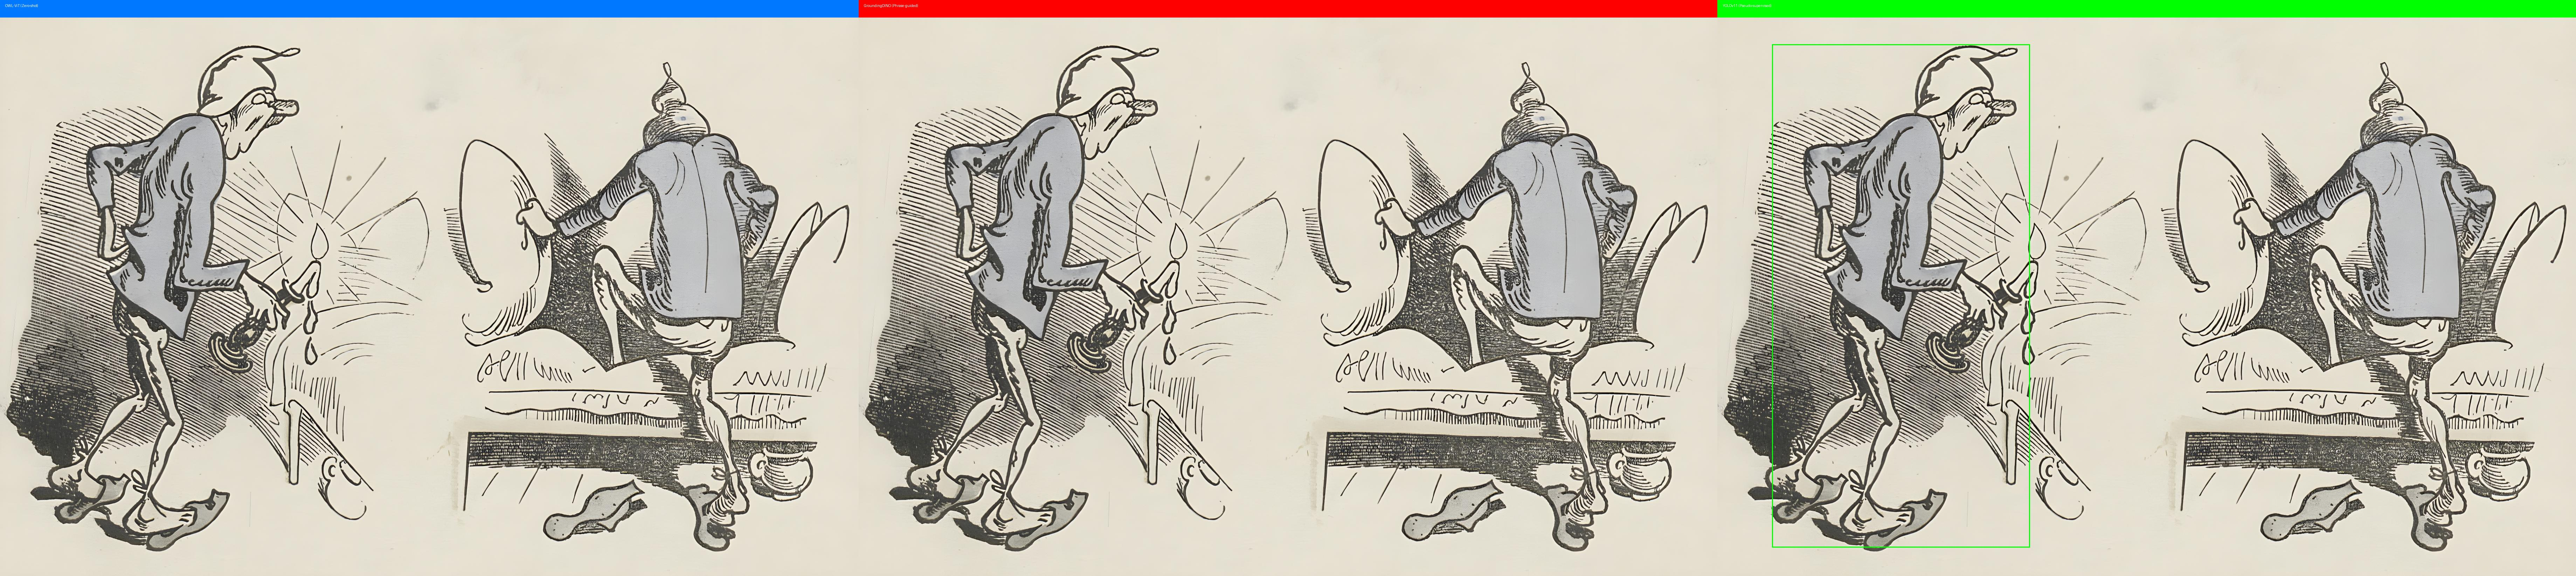
\includegraphics[width=\textwidth]{triptych_example_new.jpg}
\vskip 0.1cm
\tiny \textit{Generative Restoration Triptych: Raw scan $\rightarrow$ Super-resolution $\rightarrow$ Restored feature layer.}
\end{columns}
\end{frame}

\begin{frame}{A.2 AWLF v1 vs. AWLF v2 Error-Targeted Retraining}
\scriptsize
\begin{columns}[T]
\column{0.50\textwidth}
\begin{alertblock}{AWLF v1: Scene-Presence Pathology}
\begin{itemize}
  \item AWLF v1 trained on binary \textit{scene presence}.
  \item Initial reference split contained extreme positive class imbalance ($319$ positive vs $2$ negative scans; $99.4\%$ positive rate).
  \item Trivial models achieved an inflated $\text{F1} = 0.9969$ simply by predicting all positive.
\end{itemize}
\end{alertblock}

\begin{block}{AWLF v2: Error-Targeted Retraining}
\begin{itemize}
  \item Target redefined strictly as classification failure: $y_i = \mathbb{I}[\operatorname{sign}(S_{\text{fusion},i}{\ge}0.5) \neq y_{\text{expert},i}]$.
  \item In-sample, 5-fold CV on $C_1$: $\text{ROC-AUC} = 0.9896$.
  \item \textbf{Group-level held-out} (Slide 3.8): $\text{ROC-AUC} = \mathbf{0.6669}$ --- the honest generalization estimate.
\end{itemize}
\end{block}

\column{0.46\textwidth}
\centering
\includegraphics[width=0.92\textwidth]{exp20_error_awlf_roc_curve.png}
\vskip 0.1cm
\tiny \textit{AWLF v2 In-Sample 5-Fold CV ROC Curve ($C_1$, $\text{ROC-AUC} = 0.9896$).}
\end{columns}
\end{frame}

\begin{frame}{A.3 Semantic Ambiguity vs. Spatial Coordinate Disagreement}
\footnotesize
\begin{columns}[T]
\column{0.50\textwidth}
\begin{alertblock}{The Bounding-Box Error Paradox}
Using raw spatial detector confidence to detect human errors yields \evidence{$\text{ROC-AUC} = 0.4655$} (worse than random chance). Foundation detectors draw tight boxes with high confidence while misclassifying historical semantics.
\end{alertblock}

\begin{block}{Exp 31 Spatial Meta-Learner Resolution}
Training a Gradient-Boosted Meta-Learner on $C_2$ integrating IoU, box area, entropy, and aspect ratio variance resolves spatial layout ambiguity (\evidence{$\text{ROC-AUC} = 0.4655 \rightarrow \mathbf{0.6759 \pm 0.130}$}, 5-fold CV std).
\end{block}

\column{0.46\textwidth}
\centering
\includegraphics[width=\textwidth]{exp31_meta_learner_roc.png}
\vskip 0.1cm
\tiny \textit{Spatial Meta-Learner Error Detection ROC Curve ($\text{ROC-AUC} = 0.6759$).}
\end{columns}
\end{frame}

\begin{frame}{A.4 Tier 1 Agent Ablation and Complementarity}
\footnotesize
This is a \emph{model-level} ablation of the four architectural Tier 1 models (Object, Scene, VLM, OCR), distinct from the $U_{\text{SAA}}$ disagreement proxy itself (which uses Object, Agreement, Scene, VLM -- Slide 2.6). Tier 2 curation agents and auxiliary prototype tooling feed neither (full deployment corpus $C_0$, $n=12{,}110$):

\begin{table}[!htbp]
\centering
\scriptsize
\begin{tabular}{lcc}
\toprule
\textbf{Ablated Component} & \textbf{Mean $\sigma$} & \textbf{$\Delta$ vs.\ Full} \\
\midrule
\textbf{Full Tier 1 Ensemble} & \textbf{0.2452} & --- \\
\midrule
Remove Spatial Grounding (YOLOv11+SAM) & 0.2499 & $+0.0047$ \\
Remove Scene Classification (SigLIP) & 0.2214 & $-0.0238$ \\
Remove VQA (LLaVA-OneVision) & 0.2528 & $+0.0076$ \\
Remove Grounded OCR (Kosmos-2.5) & 0.1995 & $-0.0457$ \\
\bottomrule
\end{tabular}
\end{table}

\begin{block}{\scriptsize Reading the Result}
\scriptsize Removing OCR causes the largest \emph{drop} in disagreement: OCR is near-uncorrelated with the other three ($r\le0.07$, Slide 3.4), so it contributes the most independent variance. Removing spatial grounding or VQA (the most correlated pair, $r=0.70$) slightly \emph{increases} disagreement instead.
\end{block}
\end{frame}

\begin{frame}{A.5 Local vs.\ Frontier Critic: Withdrawn Claim, Real Replacement}
\scriptsize
\begin{columns}[T]
\column{0.50\textwidth}
\begin{alertblock}{Withdrawn: the ``Measured'' F1 Gap Was Hardcoded}
\scriptsize Contradiction F1 = 0.812 (local) vs.\ 0.965 (frontier), presented as measured on $C_4, n{=}100$ -- traced to \texttt{compare\_coordinators.py}: both are literal constants in a no-API-keys fallback branch. No F1 is computed anywhere; no gold labels exist for one. Withdrawn, with the routing-curve figure calibrated to it.
\end{alertblock}

\begin{block}{Real Replacement: Same-Model Critic Flag Rate}
\scriptsize Same Primary-then-Critic protocol, real inference:
\begin{itemize}
  \item \textbf{Local} (LLaVA-OneVision, $n=25$): \textbf{0/25} flagged.
  \item \textbf{Stronger same-model approx.} (Gemini Flash-Lite, $n=10$): \textbf{1/10} flagged, genuine catch.
\end{itemize}
\end{block}

\column{0.46\textwidth}
\begin{block}{What This Does and Doesn't Show}
\scriptsize Stronger models catch more of their own errors under re-prompting -- but this is still same-model self-review, not the documented cross-model pair (Gemini proposes, Claude audits). That genuine independence test remains \textbf{unrun} (Anthropic key lacked credit). The frontier design's rationale (disjoint weights can't share a blind spot) stands as an argument, not yet a measurement.
\end{block}
\begin{block}{Latency \& Cost (Unaffected)}
\scriptsize Local: \$0.00, self-hosted. Frontier: $\approx\$0.85$/1k images -- independent of the withdrawn F1 claim.
\end{block}
\end{columns}
\end{frame}

\begin{frame}{A.6 External Cross-Depiction Benchmark: PeopleArt ($n=4,778$)}
\footnotesize
\begin{columns}[T]
\column{0.52\textwidth}
\begin{block}{Cross-Style Generalization ($n=4,778$ Images, 43 Styles)}
\scriptsize
\resizebox{\linewidth}{!}{%
\begin{tabular}{lccc}
\toprule
\textbf{Style Category} & \textbf{Precision} & \textbf{Recall} & \textbf{F1-Score} \\
\midrule
Photo & 0.875 & 0.915 & \textbf{0.878} \\
Realism & 0.840 & 0.874 & 0.835 \\
Impressionism & 0.888 & 0.944 & 0.880 \\
Cubism & 0.836 & 0.834 & 0.831 \\
Cartoon & 0.706 & 0.680 & 0.673 \\
\bottomrule
\end{tabular}%
}
\end{block}

\begin{block}{Key Generalization Finding}
\scriptsize
Real YOLO detection degrades gracefully as style diverges from photorealism, to Cartoon ($F_1=0.673$). \textit{A per-style ``uncertainty'' figure shown here previously used hardcoded constants, not real VLM output -- withdrawn (audit).}
\end{block}

\column{0.44\textwidth}
\centering
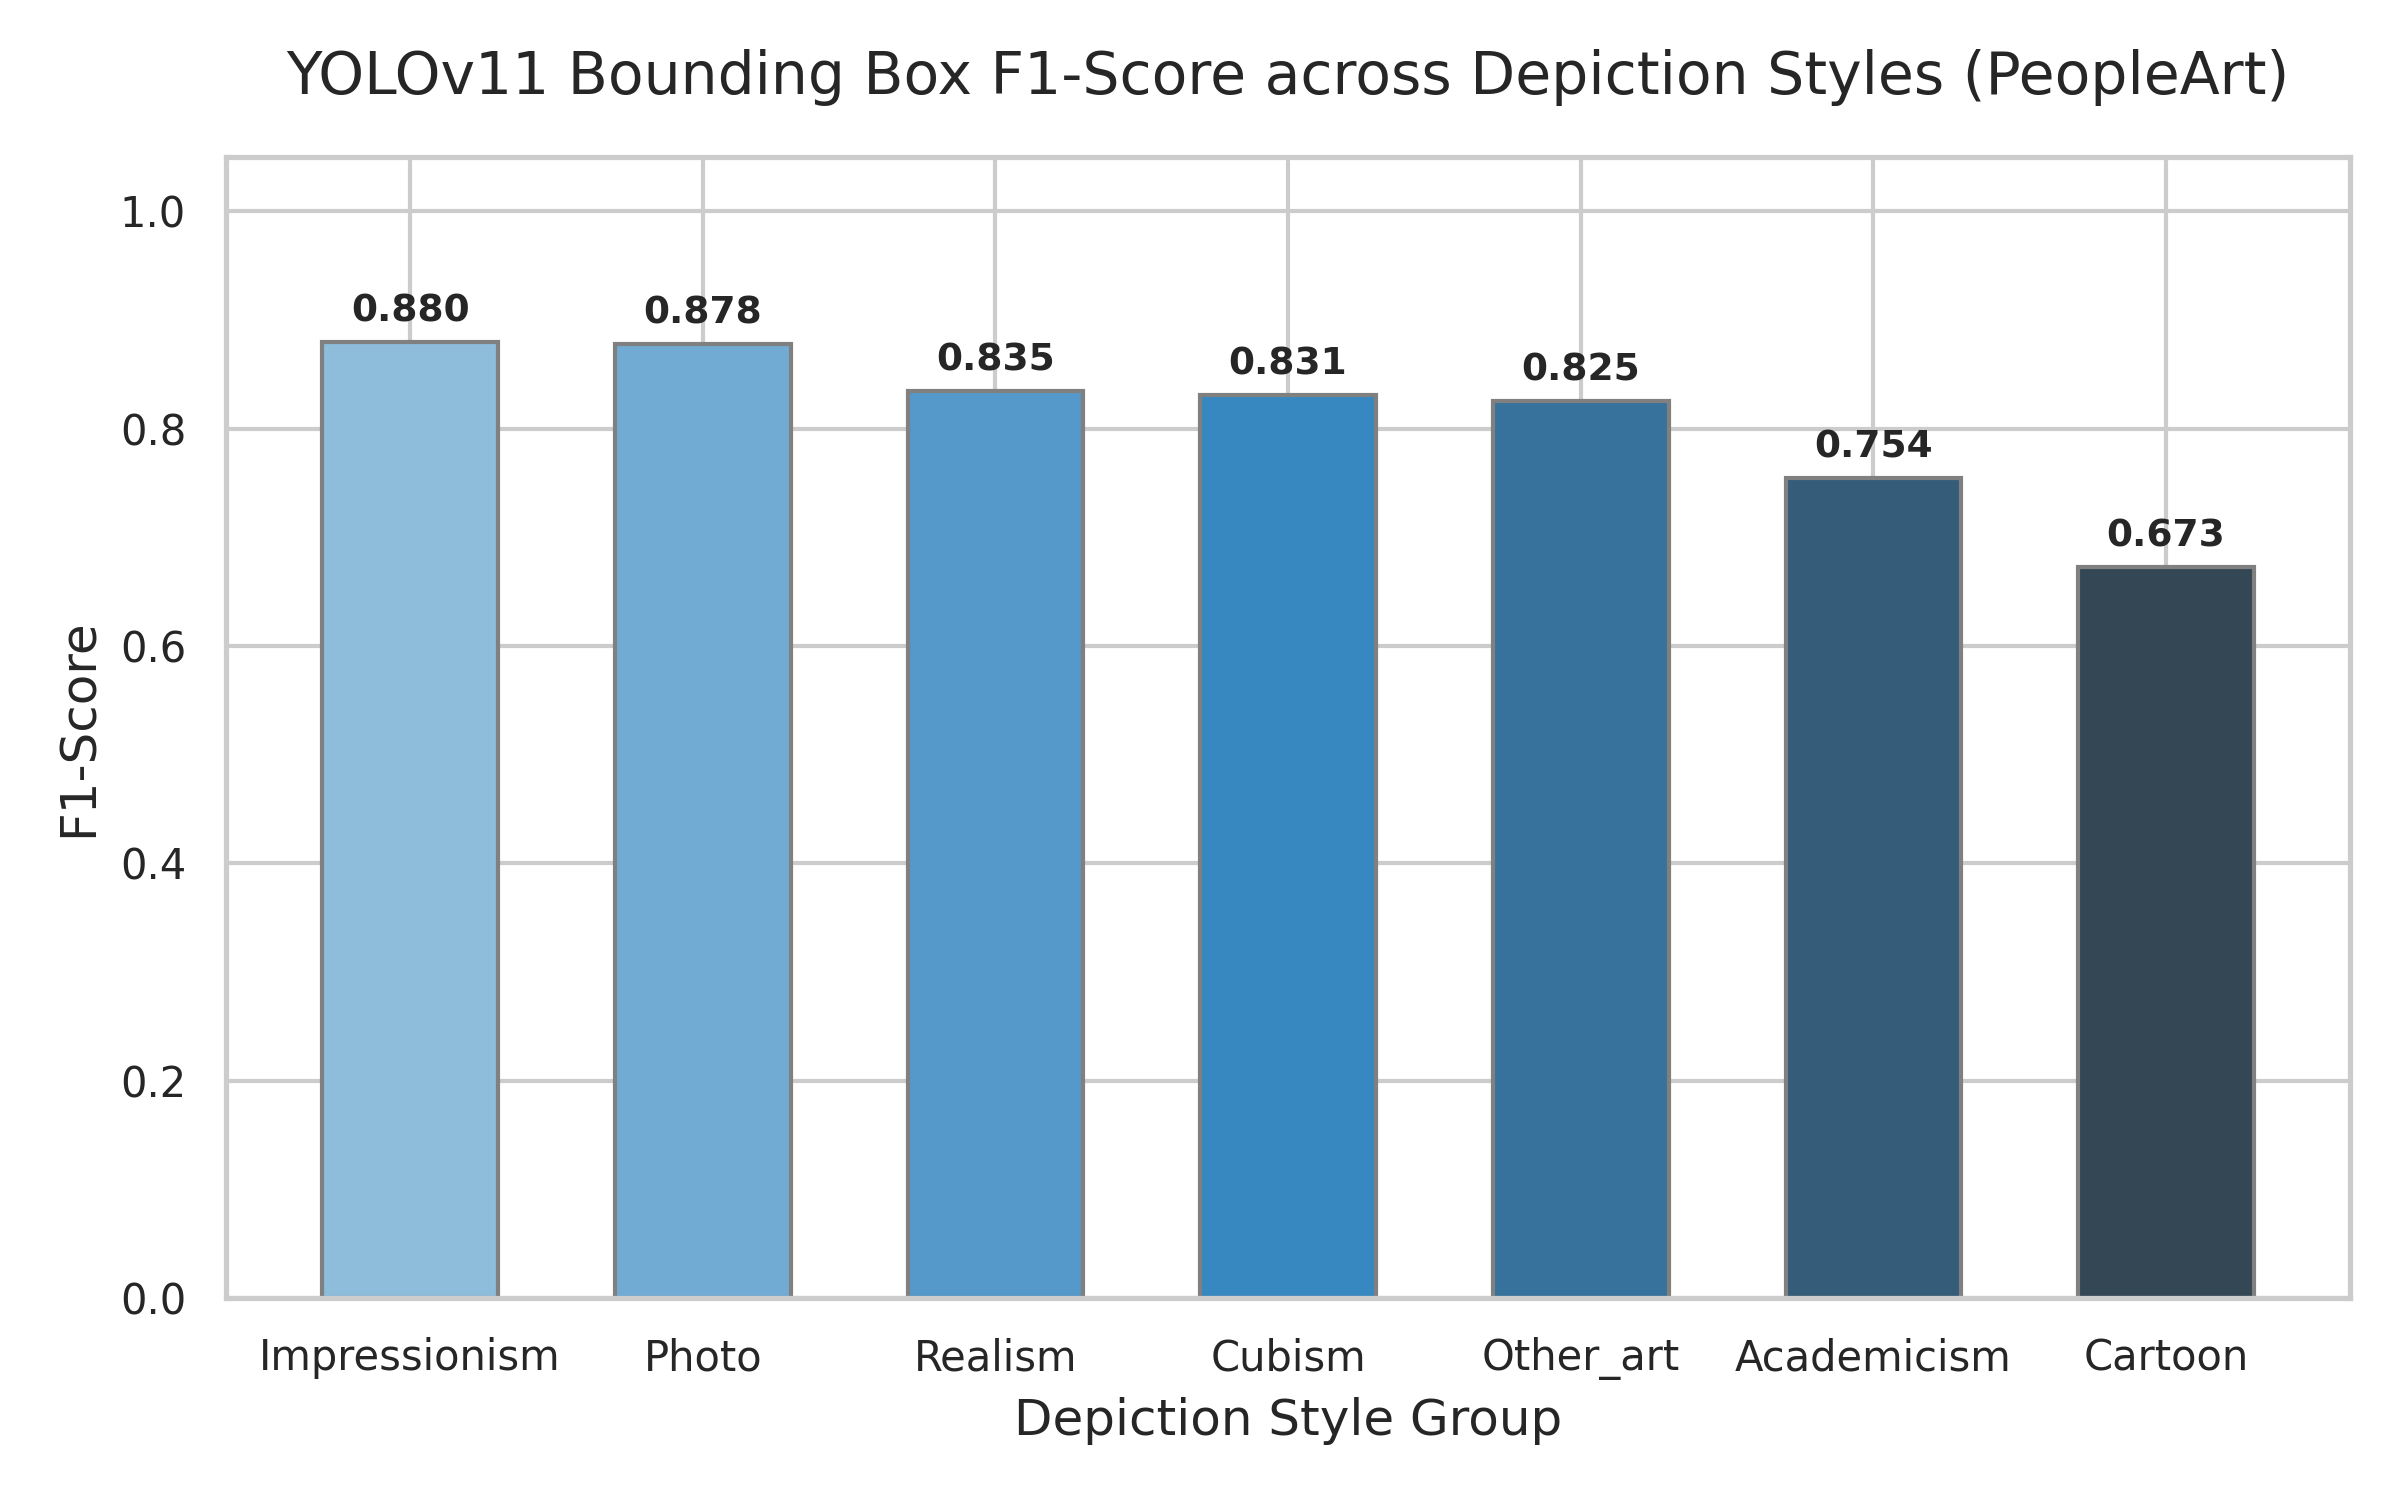
\includegraphics[width=\textwidth]{peopleart_style_f1.png}
\vskip 0.1cm
\tiny \textit{PeopleArt F1-Score by Style (real YOLO detections vs.\ ground truth).}
\end{columns}
\end{frame}

\begin{frame}{A.7 Cross-Institutional Europeana Transfer Pilot ($C_5, n=24$)}
\scriptsize
\begin{columns}[T]
\column{0.50\textwidth}
\begin{block}{Genuine Europeana Open Culture API Pilot}
Two earlier ``Europeana'' attempts did not hold up under audit: one generated VLM/scene scores via \texttt{np.random} instead of real inference; the other used \emph{no Europeana data} -- its ``30 images'' were verified ordinary Colibri images. Both withdrawn.
\begin{itemize}
    \item \textbf{Re-run for real}: 24 images live-downloaded from the Europeana API, 10 verified institutions.
    \item All 4 Tier 1 signals genuinely measured (deployed weights/prompts): YOLO+SAM, SigLIP, Kosmos-2.5, LLaVA-OV via vLLM.
    \item SAA fusion \textbf{0.332} vs.\ Colibri's \textbf{0.762} -- real, substantial domain-shift response.
    \item Ground truth pending -- annotation template ready for human labeling.
\end{itemize}
\end{block}

\column{0.44\textwidth}
\centering
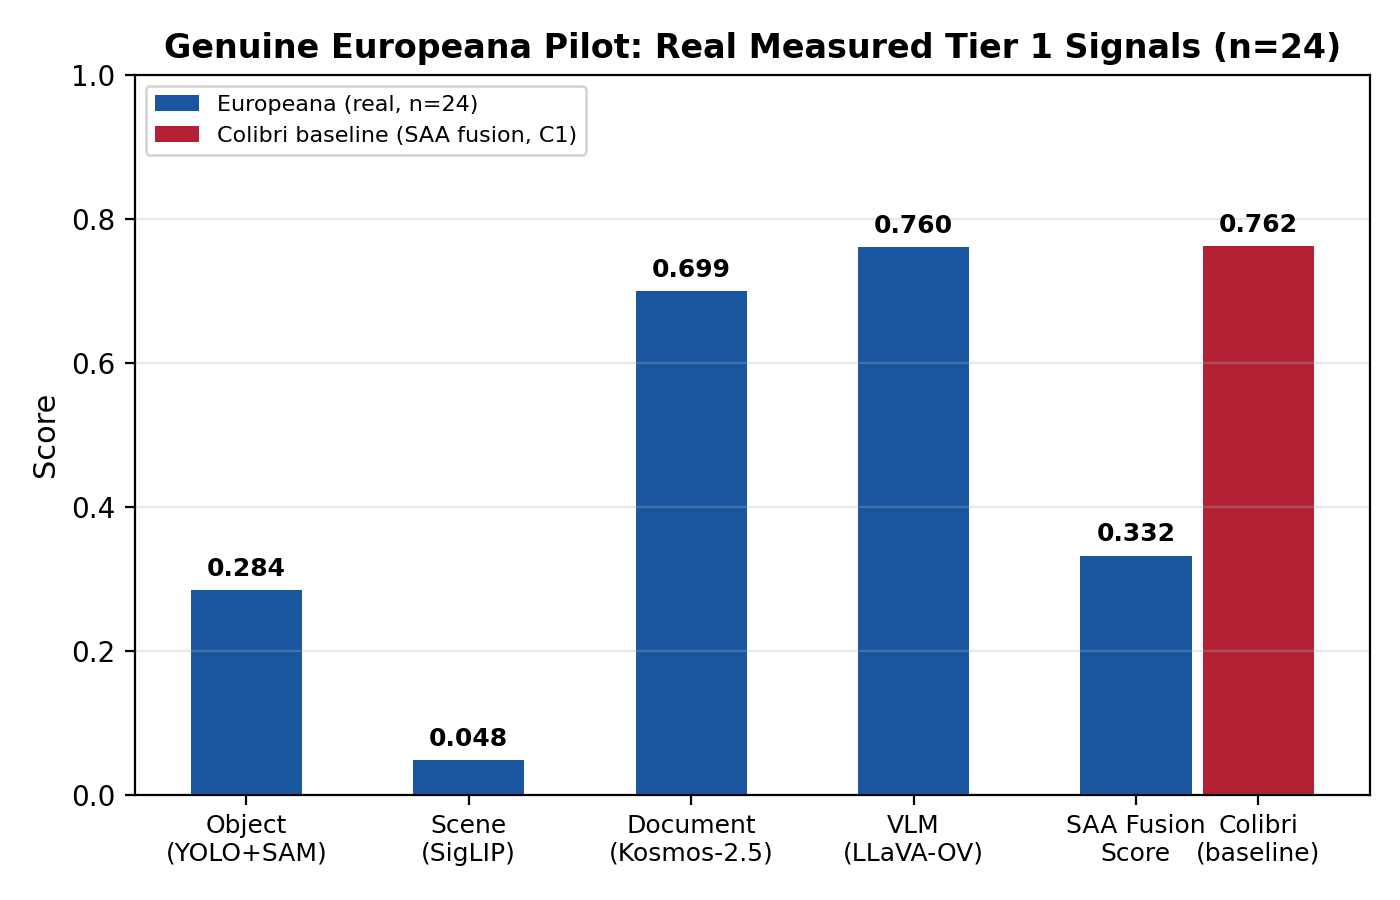
\includegraphics[width=\textwidth]{europeana_real_pilot_signals.png}
\vskip 0.1cm
\tiny \textit{Real measured Tier 1 signals on genuine Europeana images ($n=24$) vs.\ Colibri baseline.}
\end{columns}
\end{frame}

\begin{frame}{A.8 Hardware Resource Consumption \& Inference Latency}
\tiny
\centering
\textit{Deployment reference figures, not a methodological contribution -- informal single-image timings, no dedicated benchmark script/log exists. A YOLOv11 spot-check found raw forward-pass time near the table's $0.02$s, but end-to-end latency (incl.\ I/O, pre/post-processing) measured $3$--$8\times$ higher; other rows not independently re-measured.}
\vskip 0.2cm
\begin{table}[!htbp]
\caption{Hardware Resource Consumption and Per-Stage Latency (NVIDIA RTX A6000 48GB).}
\begin{tabular}{lrr}
\toprule
\textbf{Pipeline Stage / Model Backbone} & \textbf{VRAM Consumption} & \textbf{Latency / Image} \\
\midrule
CycleGAN Domain Translation & 4.2 GB & 0.15s \\
Real-ESRGAN $4\times$ Upscaling & 8.5 GB & 0.45s \\
Stable Diffusion Img2Img Refinement & 12.1 GB & 3.20s \\
Florence-2 Grounded Detection & 18.0 GB & 1.20s \\
GroundingDINO Object Detection & 22.4 GB & 2.10s \\
LLaVA-OneVision 7B VQA Reasoning & 34.2 GB & 15.00s \\
\textbf{YOLOv11 Distilled Local Inference} & \textbf{1.8 GB} & \textbf{0.02s} \\
\bottomrule
\end{tabular}
\end{table}

\begin{block}{Deployability Highlight}
The distilled student detector runs at \textbf{0.02s/image} ($750\times$ faster than LLaVA 7B), enabling real-time deployment on institutional archive servers.
\end{block}
\end{frame}

\begin{frame}{A.9 Reproducibility Spot-Checks (Not a Full Re-Verification)}
\scriptsize
A dedicated spot-check script reproduces a handful of specific intermediate numbers from source data. These are auxiliary sanity checks on isolated computations, not a re-derivation of every headline figure in this thesis (the SAA/CRC/clean-holdout numbers are produced by the main experiment pipeline, not this script):

\begin{table}[!htbp]
\centering
\begin{tabular}{lll}
\toprule
\textbf{Spot-Check} & \textbf{Recomputed Value} & \textbf{Status} \\
\midrule
YOLO-alone error detection ($C_1$)\tiny{$^\dagger$} & $0.9920$ & \textcolor{PrismGreen}{\checkmark\ reproduced} \\
\textit{Drawing}-class Deep Dive (YOLO vs VLM) & $0.5817$ / $0.8381$ & \textcolor{PrismGreen}{\checkmark\ reproduced} \\
Triage Overlap (Top 10\%, Jaccard) & $0.9739$ & \textcolor{PrismGreen}{\checkmark\ reproduced} \\
\bottomrule
\end{tabular}
\end{table}
\tiny{$^\dagger$This evaluates whether YOLO alone mispredicts -- a different target from the fusion-score error task behind the headline $0.9724$/$0.9726$ figures; the two numbers are not directly comparable.}

\begin{alertblock}{Two Corrections Applied Before This Defense}
\textbf{(1)} An earlier draft's ``dual-annotator Cohen's Kappa'' claim ($\kappa=0.8031$) traced to a script explicitly generating \textbf{simulated} two-rater data (docstring: \textit{``Creates simulated data ... to test Cohen's Kappa logic''}) --- removed entirely. \textbf{(2)} A prior ``AWLF out-of-sample AUROC=0.7868, C3 n=2,000'' claim was found to actually evaluate a 40\% split of $C_1$ ($n{\approx}321$) on the discredited scene-presence target, not the described error-detection target on $C_3$ --- its matching F1$=0.9969$ is a trivial artifact (an always-positive classifier gets the identical score). That legacy computation is still mechanically reproducible from source (it is not itself in the table above, precisely because it is not a validation of a thesis claim) but has been superseded by the group-level held-out evaluation, next slide.
\end{alertblock}
\end{frame}

\begin{frame}{A.10 Game-Theoretic Shapley Attribution (Backup)}
\footnotesize
\begin{columns}[T]
\column{0.50\textwidth}
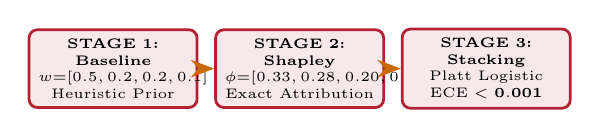
\begin{tikzpicture}[
  node distance=0.25cm and 0.2cm,
  every node/.style={font=\tiny},
  stagebox/.style={draw=HildesheimRed, fill=PrismRed!10, rounded corners=3pt, align=center, text width=1.9cm, minimum height=0.9cm, line width=1pt},
  arrow/.style={->, >=Stealth, line width=1.2pt, PrismOrange}
]
\node[stagebox] (s1) {\textbf{STAGE 1: Baseline}\\$w{=}[0.5,0.2,0.2,0.1]$\\Heuristic Prior};
\node[stagebox, right=of s1] (s2) {\textbf{STAGE 2: Shapley}\\$\phi{=}[0.33,0.28,0.20,0.19]$\\Exact Attribution};
\node[stagebox, right=of s2] (s3) {\textbf{STAGE 3: Stacking}\\Platt Logistic\\$\mathbf{\text{ECE} < 0.001}$};

\draw[arrow] (s1) -- (s2);
\draw[arrow] (s2) -- (s3);
\end{tikzpicture}

\vskip 0.2cm
\begin{block}{Exp 30 Shapley Attribution Results}
LLaVA-OneVision 7B ($\phi_1 = 0.330, 33.0\%$) and SAA Core ($\phi_2 = 0.283, 28.3\%$) provide over $61\%$ of total diagnostic signal.
\end{block}
\begin{alertblock}{\scriptsize Not the Deployed Weighting}
\scriptsize This is a supplementary interpretability study. Every result elsewhere in this thesis uses the fixed heuristic weights ($w=[0.6,0.2,0.2]$), not these Shapley values -- Shapley attributions quantify contribution to a defined coalitional objective, not independent causal correctness.
\end{alertblock}

\column{0.46\textwidth}
\centering
\includegraphics[width=\textwidth]{exp30_shapley_fusion_bars.png}
\vskip 0.1cm
\tiny \textit{Game-Theoretic Shapley Attribution Weights ($\phi_i$).}
\end{columns}
\end{frame}

% ==========================================================================
% REFERENCES
% ==========================================================================
\begin{frame}[allowframebreaks]{References}
\tiny
\begin{thebibliography}{10}
\bibitem{zhu2017} J.-Y. Zhu, T. Park, P. Isola, and A. A. Efros, ``Unpaired Image-to-Image Translation using Cycle-Consistent Adversarial Networks,'' in \textit{ICCV}, 2017.
\bibitem{realesrgan2021} X. Wang, L. Xie, C. Dong, and Y. Shan, ``Real-ESRGAN: Training Real-World Blind Super-Resolution with Pure Synthetic Data,'' in \textit{ICCVW}, 2021.
\bibitem{rombach2022} R. Rombach, A. Blattmann, D. Lorenz, P. Esser, and B. Ommer, ``High-Resolution Image Synthesis with Latent Diffusion Models,'' in \textit{CVPR}, 2022.
\bibitem{groundingdino2023} S. Liu et al., ``Grounding DINO: Marrying DINO with Grounded Pre-Training for Open-Set Object Detection,'' in \textit{ECCV}, 2023.
\bibitem{llava_onevision2024} B. Li et al., ``LLaVA-OneVision: Easy Visual Task Transfer,'' \textit{arXiv preprint arXiv:2408.03326}, 2024.
\bibitem{shapley1953} L. S. Shapley, ``A Value for n-Person Games,'' \textit{Contributions to the Theory of Games}, 2(28):307--317, 1953.
\bibitem{angelopoulos2023} A. N. Angelopoulos and S. Bates, ``Conformal Prediction: A Gentle Introduction,'' \textit{Foundations and Trends in Machine Learning}, 16(4):494--591, 2023.
\end{thebibliography}
\end{frame}

\end{document}
